\section{Введение}

В этой вводной лекции рассматривается вопрос о том, на каком этапе и какие численные методы возникают при обработке экспериментальных данных (ЭД).

Начнём с конкретного примера. В 1881 году Д.И.\,Менделеев исследовал зависимость растворимости $NaNO_{2}$ в воде от температуры. Были получены следующие данные:

\begin{table}[h]
	\small
	\caption{Зависимость растворимости соли от температуры в эксперименте Менделеева.}
	\label{table:mendeleev}
	\begin{tabular}{ p{0.25\textwidth} *{10}{|c} }

		T (температура), °C & 0 & 4 & 10 & 15 & 21& 29& 36& 51&68 & x \\
		\hline
		Масса $NaNO_{2}$ в 100~мл воды, г&
		66,7&71,0&76,3&80,6&85,7&99,4&99,4&113,6&125,1& y \\

	\end{tabular}
	
\end{table}

Это типичный пример исходных экспериментальных данных -- конечная таблица $x_i | y_i, i=1\dots n$. Задача состоит в том, чтобы найти зависимость $y = f(x)$ по этим данным. В рассматриваемом примере предполагается, что $f(x)$ неизвестна и предполагается, что $y_i = f(x_i) + \varepsilon _i$, где $\varepsilon _ i$ -- ошибки.

Что касается ошибок, то мы будем предполагать, что известна величина $\varepsilon$ такая, что с нужной вероятностью $|\varepsilon _i| \leq \varepsilon$ и $\varepsilon$ много меньше наблюдаемых значений ($\varepsilon \ll y_i$). В частности, если $\varepsilon_i$ независимые, одинаково распределенные случайные величины с нулевым средним $\langle \varepsilon_i \rangle = 0$ и дисперсией $\langle \varepsilon^2 \rangle$, то $\varepsilon \sim \sqrt{\langle \varepsilon^2 \rangle }$. В более общем случае $\varepsilon$ характеризуется величиной доверительного интервала. 

Таким образом, предполагается, что из априорных соображений или путем статистической обработки мы определили величину $\varepsilon$. Это всё, что нам нужно от статистики, и вопросы статистической обработки ЭД в лекциях рассматриваться не будут.



Если представить данные Д.И.\,Менделеева графически, то возникает картина, схематически представленная на рисунке \ref{fig:1.1}. 
\begin{figure}[h]
	\centering
 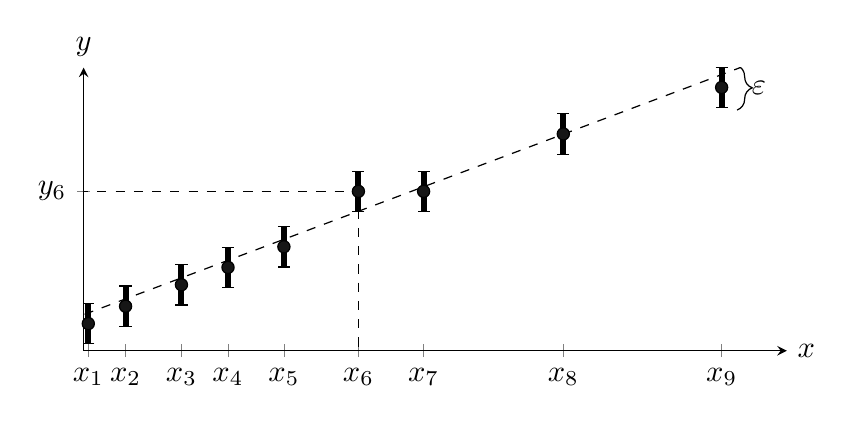
\begin{tikzpicture}[scale=1.1]
 \selectcolormodel{gray}
      \begin{axis}[%
      width = 0.8\textwidth,
      height = 0.4\textwidth,
        xmin=-0.5,
        xmax=75,
        ymax=130,
        ymin=60,
        axis y line*=left,
        axis x line*=bottom,
         axis lines = left,
       xtick = {0,4, 10, 15, 21, 29, 36, 51, 68},
        xticklabels = {$x_1$,$x_2$,$x_3$, $x_4$, $x_5$, $x_6$, $x_7$, $x_8$, $x_9$},
        ytick={99.4},
        yticklabels = {$y_6$},
        ylabel = {$y$}, ylabel style={rotate=-90},
        xlabel = {$x$},
        every axis x label/.style={
    		at={(ticklabel* cs:1.0)},
   			anchor=west,
			},
		every axis y label/.style={
    		at={(ticklabel* cs:1.0)},
    		anchor=south,
			},
      ]
        \addplot+[color=black, fill=black, only marks][error bars/.cd,y dir=both,y explicit, error bar style={line width=2pt}] coordinates {%
          (0,66.7) +- (0,5)
          (4,71.0) +- (0,5)
          (10,76.3) +- (0,5)
          (15,80.6) +- (0,5)
          (21,85.7) +- (0,5)
          (29,99.4) +- (0,5)
          (36,99.4) +- (0,5)
          (51,113.6) +- (0,5)
          (68,125.1) +- (0,5)

        };
        \addplot[dashed] coordinates {(-1, 99.4) (29, 99.4 )};
        \addplot[dashed] coordinates {(29, 99.4) (29, 60)};
        \addplot[dashed] coordinates {(-0.4, 69) (70, 130)}; 
        \draw [decorate, decoration={brace,amplitude=5pt,raise=2pt,mirror}] 
        (69,119.5) -- (69,130.5);
        \node[] at (72,125) {$\varepsilon$};
             \end{axis}
    \end{tikzpicture}
    \caption{Экспериментальные данные, представленные в графическом виде.}
    \label{fig:1.1}
\end{figure}

Эта картина позволяет предположить, что исходная зависимость имеет вид 
\begin{equation}
	y = f(x) = ax + b.
\end{equation}
 Возникает вопрос -- как определить величины $a$ и $b$?  Правильная (с точки зрения математической статистики) стратегия состоит в применении метода наименьших квадратов (МНК). Согласно этому методу величины $a$ и $b$ ищутся  из условия 
 \begin{equation}
	Q(a, b) = \sum^n_{i=1}{(a+bx_i -y_i)^2} = \min_{a,b}
\end{equation}

Так как величина $Q(a,b)$ квадратична по $a,b$, то условия
\begin{equation}
	\frac{\partial Q}{\partial a} = 0,    \frac{\partial Q}{\partial b} = 0
\end{equation}
приводят к системе из двух линейных уравнений. Их решение $a = 67,5, b = 0,87$ нашел Д.И.\,Менделеев. Необходимо ещё проверить, что для функции $f(x) = 67,5 + 0,87x$ выполняются условия $|f(x_i) - y_i| < \varepsilon$ и убедиться в том, что величины $a,b$ мало меняются при замене $y_i$ на $y_i = \varepsilon _i$. Если это так, то задача решена и при этом никаких численных методов нам не понадобилось. Это связано с тем, что зависимость простая (всего два параметра) и число измерений невелико. В случае более сложной зависимости возникает картина, представленная на следующем рисунке \ref{fig:1.2}.


\begin{figure}[h]
	\centering
 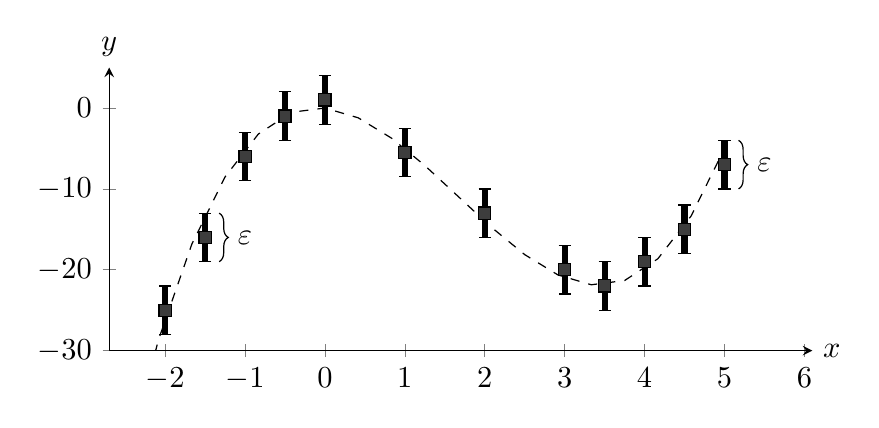
\begin{tikzpicture}[scale=1.1]
 \selectcolormodel{gray}
      \begin{axis}[%
      width = 0.8\textwidth,
      height = 0.4\textwidth,
        xmin=-2.7,
        xmax=6.1,
        ymax=5,
        ymin=-30,
        axis y line*=left,
        axis x line*=bottom,
        axis lines = left,
%        xtick = {0},
%        xticklabels = {$x_1$},
%        ytick={99.4},
%        yticklabels = {$y_6$},
        ylabel = {$y$}, ylabel style={rotate=-90},
        xlabel = {$x$},
        every axis x label/.style={
    		at={(ticklabel* cs:1.0)},
   			anchor=west,
			},
		every axis y label/.style={
    		at={(ticklabel* cs:1.0)},
    		anchor=south,
			},
      ]
        \addplot [mark=none, dashed]{x^3 - 5*x^2 - x };
        \addplot+[color=black, fill=black, only marks][error bars/.cd,y dir=both,y explicit, error bar style={line width=2pt}] coordinates {  
        (-2, -25) +- (0, 3)
        (-1.5, -16) +- (0, 3)
        (-1, -6) +- (0, 3)
        (-0.5, -1) +- (0, 3)
        (0, 1) +- (0, 3)
        (1, -5.5) +- (0, 3)
        (2, -13) +- (0, 3)
        (3, -20) +- (0, 3)
        (3.5, -22) +- (0, 3)
        (4, -19) +-(0, 3)
        (4.5, -15) +- (0, 3)
        (5, -7) +- (0, 3)


        };

        \draw [decorate, decoration={brace,amplitude=3pt,raise=2pt,mirror}] 
        (-1.4, -19) -- (-1.4, -13);
        \node[] at (-1, -16) {$\varepsilon$};
        
        \draw [decorate, decoration={brace,amplitude=3pt,raise=2pt,mirror}] 
        (5.1, -10) -- (5.1, -4);
        \node[] at (5.5, -7) {$\varepsilon$};
        
        
        
             \end{axis}
    \end{tikzpicture}
    \caption{Сложная экспериментальная зависимость, представленная в графическом виде.}
    \label{fig:1.2}
\end{figure}


В этом случае можно попытаться искать зависимость в виде 
\begin{equation} \label{eq:representation}
	f(x) = a_1 \varphi _1(x) + a_2 \varphi _2(x) + \dots + a_m \varphi _1(m),
\end{equation}
где $\varphi _k(x)$ --известные функции, например
\begin{equation}
	\varphi _k(x) = x^{k-1},  k = 1 \dots m
\end{equation}

Согласно МНК величины $a_1 \dots a_m$ ищутся из условия

 \begin{equation}
	Q(a_1 \dots a_m) = \sum^n_{i=1}{(f(x_i) -y_i)^2} = \min_{a_1 \dots a_m}
\end{equation}

и определяются исходя из полученной системы из $m$ линейных уравнений.

Возникают следующие вопросы:
\begin{enumerate}
	\item Как выбрать функции $\varphi _k(x)$ и величины $m$;
	\item Как решать полученную систему линейных уравнений;
	\item Как определить устойчиво ли решение относительно малых изменений величин $y_i$.
\end{enumerate}


Выбирая набор функций $\varphi _k(x)$ мы должны быть уверенны, что любую зависимость можно с нужной точностью представить в виде \ref{eq:representation}. Эта задача решается в теории приближений (теории аппроксимаций) и ей посвящены 2, 3, 4 лекции. Вопросы 2,3 -- это вопросы линейной алгебры и они будут рассмотрены в 5, 6, 7, лекциях.

Выше предполагалось, что вид функции $f(x)$ неизвестен. В ряде случаев вид функции  $f(x)$ известен с точностью до конечного числа неизвестных параметров.

Рассмотрим эксперимент, в котором измеряется зависимость от времени концентрации $C(t)$ некоторого вещества, при это известно, что 
\begin{equation}
	C(t) = a_1e^{\lambda_1 t} + a_2 e^{\lambda_2 t},
\end{equation}
экспериментальные данные это таблица $x_i | y_i, i=1\dots n, x_i = t_i, y_i = C(t_i) + \varepsilon_i$. Если величины $\lambda_1, \lambda_2$ неизвестны, задача их определения из условия

 \begin{equation}
	Q(a_1,a_2,\lambda_1, \lambda_2) = \sum^n_{i=1}{(C(t_i) -y_i)^2} = \min_{a_1,a_2,\lambda_1, \lambda_2}
\end{equation}
приводит к системе нелинейных уравнений. Это задача из теории оптимизации. Здесь, по существу, идёт речь о методах решения нелинейных систем уравнений, которые будут рассмотрены в лекциях 9 и 10.

Последние две лекции будут посвящены использования преобразования Фурье в задачах обработки ЭД. Будет объяснено, что такое преобразование Фурье и его дискретные варианты (ДПФ), а также как ДПФ используется в задачах "сглаживания" ЭД и обнаружения периодических сигналов.

Чтобы ориентироваться в численных методах и использовать пакеты прикладных программ, необходимо знакомство с такими понятиями как норма функций, число обусловленности матрицы и её норма, QR и SVD разложение, неподвижная точка отображения и т.д. Все эти понятия будут введены ниже по мере их возникновения в рассматриваемых задачах.

В каждой лекции используется своя нумерация формул. При ссылках на формулы впереди указывается их номер ( 3.5 = формула 5 из лекции 3).







